\documentclass[11pt,preprint, authoryear]{elsarticle}

\usepackage{lmodern}
%%%% My spacing
\usepackage{setspace}
\setstretch{1.5}
\DeclareMathSizes{12}{14}{10}{10}

% Wrap around which gives all figures included the [H] command, or places it "here". This can be tedious to code in Rmarkdown.
\usepackage{float}
\let\origfigure\figure
\let\endorigfigure\endfigure
\renewenvironment{figure}[1][2] {
    \expandafter\origfigure\expandafter[H]
} {
    \endorigfigure
}

\let\origtable\table
\let\endorigtable\endtable
\renewenvironment{table}[1][2] {
    \expandafter\origtable\expandafter[H]
} {
    \endorigtable
}


\usepackage{ifxetex,ifluatex}
\usepackage{fixltx2e} % provides \textsubscript
\ifnum 0\ifxetex 1\fi\ifluatex 1\fi=0 % if pdftex
  \usepackage[T1]{fontenc}
  \usepackage[utf8]{inputenc}
\else % if luatex or xelatex
  \ifxetex
    \usepackage{mathspec}
    \usepackage{xltxtra,xunicode}
  \else
    \usepackage{fontspec}
  \fi
  \defaultfontfeatures{Mapping=tex-text,Scale=MatchLowercase}
  \newcommand{\euro}{€}
\fi

\usepackage{amssymb, amsmath, amsthm, amsfonts}

\def\bibsection{\section*{References}} %%% Make "References" appear before bibliography


\usepackage[round]{natbib}

\usepackage{longtable}
\usepackage[margin=2.3cm,bottom=2cm,top=2.5cm, includefoot]{geometry}
\usepackage{fancyhdr}
\usepackage[bottom, hang, flushmargin]{footmisc}
\usepackage{graphicx}
\numberwithin{equation}{section}
\numberwithin{figure}{section}
\numberwithin{table}{section}
\setlength{\parindent}{0cm}
\setlength{\parskip}{1.3ex plus 0.5ex minus 0.3ex}
\usepackage{textcomp}
\renewcommand{\headrulewidth}{0.2pt}
\renewcommand{\footrulewidth}{0.3pt}

\usepackage{array}
\newcolumntype{x}[1]{>{\centering\arraybackslash\hspace{0pt}}p{#1}}

%%%%  Remove the "preprint submitted to" part. Don't worry about this either, it just looks better without it:
\makeatletter
\def\ps@pprintTitle{%
  \let\@oddhead\@empty
  \let\@evenhead\@empty
  \let\@oddfoot\@empty
  \let\@evenfoot\@oddfoot
}
\makeatother

 \def\tightlist{} % This allows for subbullets!

\usepackage{hyperref}
\hypersetup{breaklinks=true,
            bookmarks=true,
            colorlinks=true,
            citecolor=blue,
            urlcolor=blue,
            linkcolor=blue,
            pdfborder={0 0 0}}


% The following packages allow huxtable to work:
\usepackage{siunitx}
\usepackage{multirow}
\usepackage{hhline}
\usepackage{calc}
\usepackage{tabularx}
\usepackage{booktabs}
\usepackage{caption}


\newenvironment{columns}[1][]{}{}

\newenvironment{column}[1]{\begin{minipage}{#1}\ignorespaces}{%
\end{minipage}
\ifhmode\unskip\fi
\aftergroup\useignorespacesandallpars}

\def\useignorespacesandallpars#1\ignorespaces\fi{%
#1\fi\ignorespacesandallpars}

\makeatletter
\def\ignorespacesandallpars{%
  \@ifnextchar\par
    {\expandafter\ignorespacesandallpars\@gobble}%
    {}%
}
\makeatother

\newlength{\cslhangindent}
\setlength{\cslhangindent}{1.5em}
\newenvironment{CSLReferences}%
  {\setlength{\parindent}{0pt}%
  \everypar{\setlength{\hangindent}{\cslhangindent}}\ignorespaces}%
  {\par}


\urlstyle{same}  % don't use monospace font for urls
\setlength{\parindent}{0pt}
\setlength{\parskip}{6pt plus 2pt minus 1pt}
\setlength{\emergencystretch}{3em}  % prevent overfull lines
\setcounter{secnumdepth}{5}

%%% Use protect on footnotes to avoid problems with footnotes in titles
\let\rmarkdownfootnote\footnote%
\def\footnote{\protect\rmarkdownfootnote}
\IfFileExists{upquote.sty}{\usepackage{upquote}}{}

%%% Include extra packages specified by user

%%% Hard setting column skips for reports - this ensures greater consistency and control over the length settings in the document.
%% page layout
%% paragraphs
\setlength{\baselineskip}{12pt plus 0pt minus 0pt}
\setlength{\parskip}{12pt plus 0pt minus 0pt}
\setlength{\parindent}{0pt plus 0pt minus 0pt}
%% floats
\setlength{\floatsep}{12pt plus 0 pt minus 0pt}
\setlength{\textfloatsep}{20pt plus 0pt minus 0pt}
\setlength{\intextsep}{14pt plus 0pt minus 0pt}
\setlength{\dbltextfloatsep}{20pt plus 0pt minus 0pt}
\setlength{\dblfloatsep}{14pt plus 0pt minus 0pt}
%% maths
\setlength{\abovedisplayskip}{12pt plus 0pt minus 0pt}
\setlength{\belowdisplayskip}{12pt plus 0pt minus 0pt}
%% lists
\setlength{\topsep}{10pt plus 0pt minus 0pt}
\setlength{\partopsep}{3pt plus 0pt minus 0pt}
\setlength{\itemsep}{5pt plus 0pt minus 0pt}
\setlength{\labelsep}{8mm plus 0mm minus 0mm}
\setlength{\parsep}{\the\parskip}
\setlength{\listparindent}{\the\parindent}
%% verbatim
\setlength{\fboxsep}{5pt plus 0pt minus 0pt}



\begin{document}



\begin{frontmatter}  %

\title{Sustainability in the Political Economy}

% Set to FALSE if wanting to remove title (for submission)




\author[Add1]{Harriet Catherine Laing}
\ead{harrietclaing@gmail.com}





\address[Add1]{University of Stellenbosch, South Africa}

\cortext[cor]{Corresponding author: Harriet Catherine Laing}

\begin{abstract}
\small{
Abstract to be written here.
}
\end{abstract}

\vspace{1cm}


\begin{keyword}
\footnotesize{
Environmental policy \sep Political economy \sep Numerical model \\
\vspace{0.3cm}
}
\end{keyword}



\vspace{0.5cm}

\end{frontmatter}



%________________________
% Header and Footers
%%%%%%%%%%%%%%%%%%%%%%%%%%%%%%%%%
\pagestyle{fancy}
\chead{}
\rhead{}
\lfoot{}
\rfoot{\footnotesize Page \thepage}
\lhead{}
%\rfoot{\footnotesize Page \thepage } % "e.g. Page 2"
\cfoot{}

%\setlength\headheight{30pt}
%%%%%%%%%%%%%%%%%%%%%%%%%%%%%%%%%
%________________________

\headsep 35pt % So that header does not go over title




\hypertarget{introduction}{%
\section{Introduction}\label{introduction}}

There have been many international environmental agreements (IEAs)
entered into between countries to reduce environmental degradation which
have fallen short of their objectives. For the non-renewable resources
within the economy to be allocated efficiently in a way that considers
sustainability for future generations requires co-operation among
countries (Buchholz \emph{et al.}, 2005). In practice, true co-operation
that is ensured by credible commitment to policy preferences is
difficult to achieve. In fact, international agreements between
countries may be counterproductive if citizens do not fully internalise
the joint impact of consumption on the probability of a climate crisis.

In this thesis, the framework from Buchholz \emph{et al.} (2005) is
employed and extended for studying the issue of international
co-operation regarding environmental policies. Their framework assumes
symmetry between two countries and that there is a trade-off between
environmental policies and gross domestic product. The paper thus
suggests countries pay each other side payments to compensate for
transboundary pollution emitted from their own country to another. Their
main result is analytically determining the global population result,
the non-cooperative result, and the bargaing outcome which lies between
the first two results.

This thesis extends the framework from Buchholz \emph{et al.} (2005) in
two novel ways. The first contribution is to create a simplified
framework to model sustainability in a formal way that enables the
incorporation of a non-linear trajectory of resource consumption over
time. If a climate crisis occurs, then the path of consumption is
permanently shifted with severely reduced consumption options for the
next period. The second contribution of this thesis is to use a
numerical modelling approach. This approach enables the study of more
nuanced questions and specifically, in this case the inclusion of
asymmetries between countries which could otherwise not be accomplished
in a purely analytical model approach.

Albeit that to replicate the full analysis that Buchholz \emph{et al.}
(2005) conducts with this new framework is beyond the scope of this
thesis, the following results are found. The outcomes under perfect
cooperation in the global democracy are determined, and the outcomes
under a fully non-cooperative interaction between a partitioned global
democracy into two countries, where each country has an elected
candidate voted in according to the voting decisions of the citizens who
take the other country's consumption decisions as given.

\emph{This yields the threat points for bargaining equilibria which is
left for future research. I show that similar results arise as in
Buchholz: When two countries elect representatives strategically, the
level of consumption chosen and hence the probability of a crisis is far
higher that what would be chosen in the cooperative environment. This
implies that any Nash bargaining solution will also be suboptimal,
although that is beyond the scope of this paper.}

\emph{Next i show how these threatpoints and final probability of crisis
depends on asymmetries in country size and opinions. (summarize the main
result explicitly here)``}

Some papers suggest that IEAs are ineffective because of strategic
voting by voters to ensure their own country's bargaining position is
stronger (Buchholz \emph{et al.}, 2005). The primary objective of this
research assignment is to model how interactions in the political
economy inhibit IEAs. Ultimately, we wish to understand how the
dominance of certain countries in the global context impacts IEAs. For
example, a country which is geographically larger than another and thus
has more voters may lead to sub-optimal outcomes in comparison to a
model considering only one large global population. Similarly, if one
country's citizens hold more optimistic beliefs about the worst case
scenario which may arise if environmental degradation passes some
threshold then this too may lead to sub-optimal outcomes.

Our paper suggests that the mechanism behind these sub-optimal outcomes
in a two-country IEA is strategic voting if voters take into account the
impact of another country's consumption level into their own best
response function. This is because our model assumes each voter receives
a random private signal that determines their beliefs about the worst
case scenario if environmental degradation crossed some threshold. These
beliefs are then mapped onto probability of crisis beliefs.

EXPLAIN STRATEGIC\ldots BELIEFS THE SAME BUT OUTCOMES DIFFERENT Thus,
strategic voting may diminish the effectiveness of IEAs. This is made
evident by the finding that when two countries are of a similar size,
the Nash equilibrium outcome yields a much higher consumption level and
probability of crisis than when one country is much larger than the
other.

If perfect co-operation cannot be ensured, then it may be better to
allow countries to unilaterally set their own environmental policies, as
this may yield greener winning political candidates, reduce pollution,
and provide a higher payoff for the median voter (Buchholz \emph{et
al.}, 2005). Buchholz \emph{et al.} (2005) investigates the sub-question
of how to bind a country to implement their true policy preferences in
an agreement, and this is still inconclusive.

The model we set up first considers the simplest case of a two-period
optimisation problem. There is a world with abundant resources, where
consumers believe that they can consume a lot today and tomorrow, and
information about the state of the world is aggregated perfectly. As we
continue to model this problem, frictions are added. For example, the
state of the world may not be aggregated correctly to the voters. For
our model, the focus is how the political system works when there is the
issue of environmental degradation. Accordingly, the literature on both
sides of the sustainability of the political economy is considered.
Namely, the literature on exhaustible resources (including the optimal
depletion thereof and the cake-eating optimisation problem) and the
political economy (including the aggregation of political information
and strategic voting).

The first specification of the state of the world will be modeled within
a global economy in which there is only one population of voters and
information is aggregated imperfectly. The second specification of the
model will introduce the two-country setting and how adjustments to the
bias of voter signals and the relative size of the countries may affect
each country's citizens' voting decisions. Thereafter, the two
specifications will be compared to each other to determine how
co-operation between countries with regards to environmental policies
may be disadvantageous for consumption and may make the probability of a
crisis more likely.

\hypertarget{literature-review}{%
\section{Literature review}\label{literature-review}}

\emph{(2400)}

The literature review for this thesis will be organised as follows.
First, the literature pertaining to the extraction of non-renewable
resources in a single economy setting is discussed. Secondly, within the
same context, the information aggregation literature is discussed.
Finally, the consideration of co-ordination across countries relating to
these issues is then discussed.

The literature which models the utilisation and extraction of
non-renewable resources began with contributions that did not
incorporate uncertainties (Pindyck, 1978). Thereafter, it developed to
consider the impact of consumption in the present period on the
resources remaining for the following period (Adler \& Treich, 2017),
and ultimately began to incorporate the possibility of consumption in
the present period as a determinant of the probability of crisis (Loury,
1978; Kumar, 2005; Lemoine \& Traeger, 2014).

Pindyck (1978) models two different optimal paths for using
non-renewable resources which depends on the initial resource endowment
and the different marginal costs of extraction for different resources.
If the initial reserve endowment is large, then this causes extraction
costs to be low and thereby the price will slowly rise over time as the
resource depletes. On the other hand, if the initial reserve has already
been depleted and there is only a small quantity remaining, both the
price and the extraction costs will be high. As reserves decline, the
production cost for using resources increases and potential profits
reduces. Accordingly, as marginal costs increase for extraction,
producers will begin to conserve non-renewable resources because the
marginal benefit thereof is smaller.

Pindyck (1978) can be incorporated into a model of sustainable
consumption by modelling that there is a cost in the future if
consumption in the present period is too high. Consumption of resources
is thus only sustainable if consumption in the present period does not
impose a cost in the next period. However, the model in this paper does
not consider the more realistic situation in which the non-renewable
resource quantities are uncertain and thus does not address the
possibility of exhausting a resource in its entirety.

Adler \& Treich (2017) consider three dimensions of climate policy to be
modelled: (i) equity, (ii) time, and (iii) risk which each impact how
risky consumption is allocated intertemporally. These three dimensions
can be interpreted as beliefs which are used in our model to inform the
optimal level of consumption and probability of crisis. The cake-eating
problem for an uncertain quantity of resources with a social planner who
allocates between the current and future generation is modelled in terms
of three different social welfare functions. The first generation is
given a determinate amount of consumption, but the second generation is
given the risky remainder. Our model also includes only the first
period's consumption as the choice variable which then impacts the
second period, but instead of first period consumption directly
impacting what is remaining for the next period, in our model
consumption impacts the probability of crisis. The methodology used is a
prioritarian social welfare function (SWF) which is the sum of some
increasing, concave function of utility for the well-being of a
generation. To find the optimal consumption allocation, Adler \& Treich
(2017) compare statics analysis for the different functions.

These aforemetioned papers, however, do not consider the uncertain
thresholds which cannot be exceeded without incurring a cost, more
specifically without altering the trajectory of an economy permanently,
such as enterring a crisis. Kemp (1976) was the first to consider the
cake-eating optimisation problem for a non-renewable resource of an
unknown size and has since been developed in the literature. Loury
(1978) investigates the optimal planning for an economy faced with two
main problems; (i) the possibility of exhaustion of the resource, and
(ii) learning about the distribution of reserves over time through
exploration and extraction activities.

Under certainty, when the size of the resource reserve is known, Loury
(1978) finds that the possibility of exhaustion occurs only
asymptotically. However, when the resource reserve quantity is of an
unknown size, the date upon which it will have been completely exploited
is also a random variable. The choice of the rate of consumption is
necessarily affected by the impact of the consumption rate on the
probability of crisis, or likelihood of reaching the tipping point. This
feature is incorporated directly into our model as the consumption in
period one which is believed to be optimal directly determines
individual's beliefs regarding the optimal probability of crisis, and
thus affects the choice of consumption.

Loury (1978) demonstrates that the possibility of premature exhaustion
alters the requirements of an optimal consumption path. The model used
in this paper specifies some minimal level of resource consumption that
is necessary to sustain an economy, which is incorporated into our model
as the lower consumption threshold. Moreover, the uncertain reserve of
resources is modelled in Loury (1978) as a random variable that is drawn
from a cumulative density function, which is a mechanism that our model
similarly employs to draw unknown values.

Kumar (2005) reconsiders Kemp's use of an infinite planning horizon by
instead using a hazard function which is defined as the probability of
reaching the climate tipping point. The paper argues that `cake-eating
under uncertainty' has two main aspects: (i) the optimal planning
horizon and (ii) the characterisation of the optimal program. The former
aspect of the (i) optimal planning horizon can be assumed to extend far
enough into the future to allow for the resource to be fully exhausted
at some point. By employing a hazard function to model the problem, the
planning horizon over which consumption of the exhaustible resource is
positive has been found to be either finite or infinite.

The main findings of Kumar (2005) are that if an uncertain resource
stock is finite and the optimal planning horizon is finite, hazard rates
increase in unbounded fashion, and marginal utility of extraction and
consumption at zero is finite. However, if an uncertain resource stock
size is unbounded, the planning horizon is infinite. Thus, the optimal
rate of extraction and consumption over time generally moves
monotonically in the opposite direction to the hazard rate.

Lemoine \& Traeger (2014) addresses the need to integrate policy with
possibility of climate tipping points into a benchmark integrated
assessment model to analyse the intertemporal trade-offs which
characterise climate policy decisions. Crossing the threshold shifts the
world permanently to a new altered system with different dynamics to the
state of the world pre-threshold. The paper demonstrates with an
analytical model that optimal policy is impacted by tipping points via
two channels; namely (the differential welfare impact (DWI) recognizes
that the present period's policy choices affect (i) welfare if a tipping
point occurs, and (ii) the probability of crossing the threshold.
Accordingly, the paper's model endogenises welfare and the probability
of a tipping point occuring, which our model incorporates.

On the political economy side of the literature, Piketty (1999) provides
a short summary of recent contributions to the literature related to
political institutions as an information-aggregation mechanism since the
first contribution by Condorcet. Other papers modelled voting behaviour
according to an individual's best response function dependent on their
own voting type and preferences (Lohmann, 1994) or dependent instead on
the voting behvaiour of others (Besley \& Coate, 1997; Buchholz, 2005).
On the other hand, Razin (2003) modelled that voters may adjust their
voting behaviour to influence either the likelihood of their candidate
getting into office or their preferred policy being implemented. Many
models of political economy include different stages to analyse how
voting impacts policies but vary according to how voters' derive utility
(Lohmann, 1994; Besley \& Coate, 1997; Razin, 2003; Buchholz \emph{et
al.}, 2005). Our model does not include voting stages explicitly, but
instead models two stages of resource consumption, and draws different
aspects from the following papers.

Condorcet was the first to posit that political institutions have a
constructive role in efficiently aggregating information in a society.
His main contribution to the literature was termed the `Condorcet Jury
Theorem' which states that under free elections, the probability that
the policy that is preferred by the majority will win by majority vote
tends to one as the number of individuals in the population tends to
infinity. This theorem posits that democracy is an efficient
information-aggregation system if it is assumed that individuals are
homogenous in both their initial prior beliefs about the state of the
world and their utility functions.

Condorcet also assumed voters vote sincerly in accordance with their
beliefs and do not engage in strategic voting. Piketty (1999) finds that
towards the end of the twentieth century, formal political models began
including information economics, and may indicate a return to the
approach of Condorcet. Extensions of the Condorcet model incorporated
the more realistic nature of information in an economy; information is
never fully integrated, but rather exists in an economy as dispersed,
incomplete and often contradictory pieces. Thus, it has since been
modelled that each individual receives a signal drawn from the same
conditional distribution, which has been used in developing our model.

Lohmann (1994) investigated the impact of the information aggregated by
political action on whether votes are more or less accurate, where
accuracy is defined in terms of reflecting voters' preferences. The
paper models that each individual has a loss function which accounts for
the loss if the policy outcome is not what the individual desired and
the private cost if the individual engaged in political action. The
equilibrium point is where an individual's political action strategy
minimises their expected loss after the political action stage. To
analyse voter behaviour, Lohmann (1994) uses game theoretical best
responses at each voting stage. For example, at the political action
stage, a voter's best response is a function of the `type' of voter that
they are and the individual preferences which they have. Similarly, our
model uses best response functions for voting behaviour but omits the
consideration of voter types, as voters are distinguished only by their
private signals.

Razin (2003) models elections with only two potential candidates in a
one-dimensional policy space. Voting behaviour is strategic as voters
are motivated by both the election and signalling implications of
voting. Election motivations refer to voters deciding to vote to
influence which candidate wins the vote, whereas signalling motivation
refers to voters voting to influence which policy the winning candidate
will implement. In our model, it is assumed instead that the winning
candidate will credibly commit to implementing their own preferred
policy and voters may engage in strategic voting to bolster their own
country's bargaining position in the two-country model. Razin (2003)
assumes that voters are privately and imperfectly informed about a
common shock which impacts voters' preferences. Voters' private signals
are drawn independently from a distribution and are conditional on the
common shock. Our model adopts the same mechanism to determine voters'
beliefs, albeit without the inclusion of a common shock to the economy.

Buchholz \emph{et al.} (2005) investigates the policy outcome which may
arise from IEAs when governments are democratically elected by citizens.
This paper considers two pertinent themes, namely the case in which a
voter may be incentivised to support a political candidate who is less
environmentally inclined than the voter's own preferences, and the case
in which the elected candidate pays no attention to environmental
policies, and thus international agreements are rendered as ineffective.
The paper argues that an efficient allocation of resources that is
sustainable requires co-operation between countries, but that there is a
far way to go before IEAs are fully enforced to function fully
cooperatively as they are intended.

According to Buchholz \emph{et al.} (2005), one possible reason for
ineffective IEAs is that voters are incentivised to deliberately support
candidates with different environmental preferences to their own in
order to improve their country's bargaining position in international
negotiations. Our paper investigates a very similar research question
and adopts a similar methodology. The methodology of Buchholz \emph{et
al.} (2005) is to use the median-voter approach with Nash bargaining in
a simple two-country model and then compare the isolationist case (in
which there is no IEA between countries) to the cooperative case (in
which there is an IEA).

The paper compares the two different cases and finds that countries will
be incentivised to improve their bargaining position in an IEA by
introducing less green policies, than they would otherwise in a
unilateral arrangement. The paper models the electoral system in a
stylised way which means that the winning candidate is determined when
they win every pairwise comparison with all other candidates and assumed
that the competing candidates have different types ranging between 0 and
1. Our model also uses the pairwise comparison for each voter to
determine which candidate would yield their highest expected utility.
However, Buchholz \emph{et al.} (2005) provides attention to varying
degrees of transboundary pollution, which refers to one country's
polluting impact on another country, whereas our paper focuses more on
the impact of varying the size of countries and introducing biased
beliefs to assess how this may impact the voting in a two-country model.

On the other hand, Besley \& Coate (1997) sets up a model of
representative democracy in which citizens have the choice to avail
themselves as candidates to run for public office. The model assumes
that candidates must credibly commit to implementing their preferred
policy if they win the election and voters then vote accordingly. Voters
derive utility from the ultimate policy outcome and the winning
candidate's identity. Voters derive disutility from the cost of running
for office if they decide to do so. There is strategic voting because
voters' voting decisions are optimal if they are a best response, given
the rest of voters' decisions. The paper defines the equilibrium policy
choice as efficient according to a Pareto optimal definition; meaning
that there are no alternative policy choices in the present period that
could increase the expected utility of all citizens conditional on
future policies that are democratic in nature.

However, this model assumes complete information. It recommends that
future research incorporates uncertainty regarding voters' preferences
and endogenises the formation of parties or candidates that run for
office. Unlike Besley \& Coate (1997) which accounts for the policy
outcome and winning candidate's identity as providing utility and the
cost of running for office as providing disutility, our model simplifies
away the cost of running for office to simply understand how
international co-operation may move countries away from better
environmental policy outcomes than if they acted unilaterally.

To conclude, this thesis models both sides of the literature discussed
in this section in a simplified way??. The interaction between two
countries which vote for how non-renewable resources should optimally be
extracted to avoid a tipping point is incorporated with the information
aggregation in the political economy. Thus, the political economy model
with consumption decisions can be extended to analyse co-ordination
between two countries in this regard.

\hypertarget{a-model-of-sustainable-consumption-in-a-global-democracy}{%
\section{A model of sustainable consumption in a global
democracy}\label{a-model-of-sustainable-consumption-in-a-global-democracy}}

\emph{(1250)}

The first specification of the model serves as a benchmark of the most
efficient information-aggregation system that may arise from majority
voting in a global democracy. There is only one population of voters.
Information is aggregated imperfectly and voters are uncertain about the
true penalty that the economy will face if consumption today exceeds
some threshold. The model is simulated in Matlab and the built-in
optimisers in the programme are used to find the optimal points. First,
the economy will be specified in a context with an unknown penalty if a
crisis occurs and then the probability of crisis will be incorporated.
Thereafter, the consumer problem and voting process will be presented.

\hypertarget{economy}{%
\subsection*{Economy}\label{economy}}
\addcontentsline{toc}{subsection}{Economy}

In order to model sustainability in the political economy, we first set
up a simple model of sustainable consumption over two periods
\(t = 1, 2\). The choice variable in this economy is consumption in
period one (\(c_1\)). Consumption in period two (\(c_2\)) is stochastic
and dependent on the value of \(c_1\) as follows. \(c_1\) is defined as
sustainable if it is below an unknown threshold value (\(\tilde{c}\)).
This is because if \(c_1\) is sustainable, then \(c_2\) can also be set
at the same level (\(c_1\) = \(c_2\)). However, if \(c_1\) is
unsustainable, and exceeds \(\tilde{c}\) in period one, then the economy
will face a climate crisis, and consumption is dramatically reduced to
some very low level (\(\underline{c}\)). As a result, \(c_2\) will be
much lower than \(c_1\) (\(c_1> \underline{c}\)). Thus, we can model
\(c_2\) as a function of \(c_1\) as follows:

\[
c_2\left(c_1\right)= \begin{cases}c_1 & \text { if } c_1 \leq \tilde{c} \\ \underline{c} & \text { otherwise }\end{cases}
\]

\hypertarget{consumers}{%
\subsection*{Consumers}\label{consumers}}
\addcontentsline{toc}{subsection}{Consumers}

The decision problem faced by consumers in the global democracy is to
maximise their lifetime utility as follows: \[
U\left(c_1\right)=u\left(c_1\right)+\mathbb{E} u\left(c_2\left(c_1\right)\right)
\]

\begin{center}
subject to $c_L \leq c_1 \leq c_H$
\end{center}

We assume that the unknown tipping point \(\tilde{c}\) is uniformly
distributed btween two known boundaries \(c_L\) and \(c_H\). In this
setting, \(c_L\) represents the safest level of consumption at which the
probability of a crisis is zero. This can be regarded as some minimal
level of consumption that is necessary to sustain an economy or the very
least amount of resources that are required to continue living (Loury,
1978). On the other hand, \(c_H\) represents the maximum consumption
value that may be consumed in period one at which the probability of
crisis is one. This can be regarded as some upper bound of consumption
possibilities where it is certain that the threshold \(\tilde{c}\) will
be reached. Due to the uncertain value of \(\tilde{c}\) that is drawn
from a uniform distribution between \(c_L\) and \(c_H\), \(c_H\) thus
represents a certainty of reaching the ``tipping point'' (Kumar, 2005;
Lemoine \& Traeger, 2014). Accordingly, if this unknown threshold
\(\tilde{c}\) is exceeded, the crisis occurs below \(c_H\).

\[
\operatorname{Pr}\left(\tilde{c} \leq c_1\right)=\left\{\begin{array}{cc}
0 & \text { if } c_1 \leq c_L \\
\frac{c_1-c_L}{c_H-c_L} & \text { if } c_1 \in\left(c_L, c_H\right] \\
1 & \text { otherwise }
\end{array}\right.
\]

We make the assumption that the utility functions of all consumers are
homogenous (Piketty, 1999) where the utility derived from consumption is
assumed to take the relative risk aversion functional form and \(\rho\)
is assumed to be set at 1.5 as follows:

\[
U(C)=\frac{c^{1-\rho}-1}{1-\rho}
\]

To introduce a role for political aggregation of private information in
the model, we assume that there are different beliefs about the severity
of the climate crisis if the tipping point is crossed. Specifically, as
in Besley \& Coate (1997), we assume that individuals differ regarding
their beliefs about the level of consumption that would be possible if
the crisis occurs (\(\underline{c}\)). These beliefs are determined by
private signals \(\hat{\underline{c}}_k\) which consumers receive. These
signals are noisy and conceal the true value of \(\underline{c}\) as
follows: \[
\hat{\underline{c}}_k=\underline{c}+\varepsilon_k
\]

\begin{center}
where  $\mathbb{E}\left(\varepsilon_k\right)=0$ 
\end{center}

We assume that these private signals \(\hat{\underline{c}}_k\) are drawn
from a distribution between \(c_L\) and \(c_H\). This is a realistic
assumption because in the real world consumers are exposed to a variety
of news sources and political action which each suggest different
probabilities for future climate outcomes (Piketty, 1999; Lohmann,
1994). Thus, information aggregation is not perfect in this model.

From the signals that are drawn randomly for each individual, there are
different associated optimal probability of crisis points. The different
signals that individuals draw determine their beliefs about which
probability of crisis is optimal, and thus lifetime utility constitutes
the utility derived from consumption in period one \(c_1\) and the
expected utility of the weighted probability average of period two
consumption as follows:

\[
U\left(c_1 \mid \hat{\underline{c}}_{k}\right)=u\left(c_1\right)+\operatorname{Pr}\left(\tilde{c} \leq c_1\right) u\left(\hat{\underline{c}}_{k}\right)+\left(1-\operatorname{Pr}\left(\tilde{c} \leq c_1\right)\right) u\left(c_1\right)
\]

In this model, the thresholds of consumption in period one are set as
exogenous, fixed parameters. The global population is set to 1000. The
set of possible consumption choices are set to 100 and are bounded
between the thresholds, which are set to \(c_L\) = 0.5 and \(c_H\) = 1.5
respectively. These choices are arbitrary, but serves as a
proof-of-concept of this numerical model structure. Future research will
extend the specifications to be more realistic or calibrated to
scientific and economic data. However, adjustable parameters are
introduced into the two-country model in the subsequent section of this
paper.

Figure 3.1 shows the cumulative distribution function of the probability
of crisis. It is curved due to the relative risk aversion functional
form. Figure 1 indicates that individuals who receive higher private
signals believe that the consumption level that is possible if the
climate crisis occurs will be higher, and thus will optimally prefer a
higher probability of the crisis occurring. An individual's optimal
probability of crisis depends on the signal provided to the individual.
The higher the signal, the higher the optimal consumption point and thus
the higher the optimal probability of crisis.

On the other hand, individuals that have been provided with information
which indicates that the climate crisis will be mild will consume more
and thus be comfortable with a higher probability of crisis. Thus,
beliefs are a key driver of consumption choices in our model. This model
builds on Besley \& Coate (1997)'s model which selects candidates
exogenously and assumes complete information within the economy. Our
model instead assumes imperfect information and unique signals that are
randomly provided to each voter.

\begin{figure}[H]

{\centering 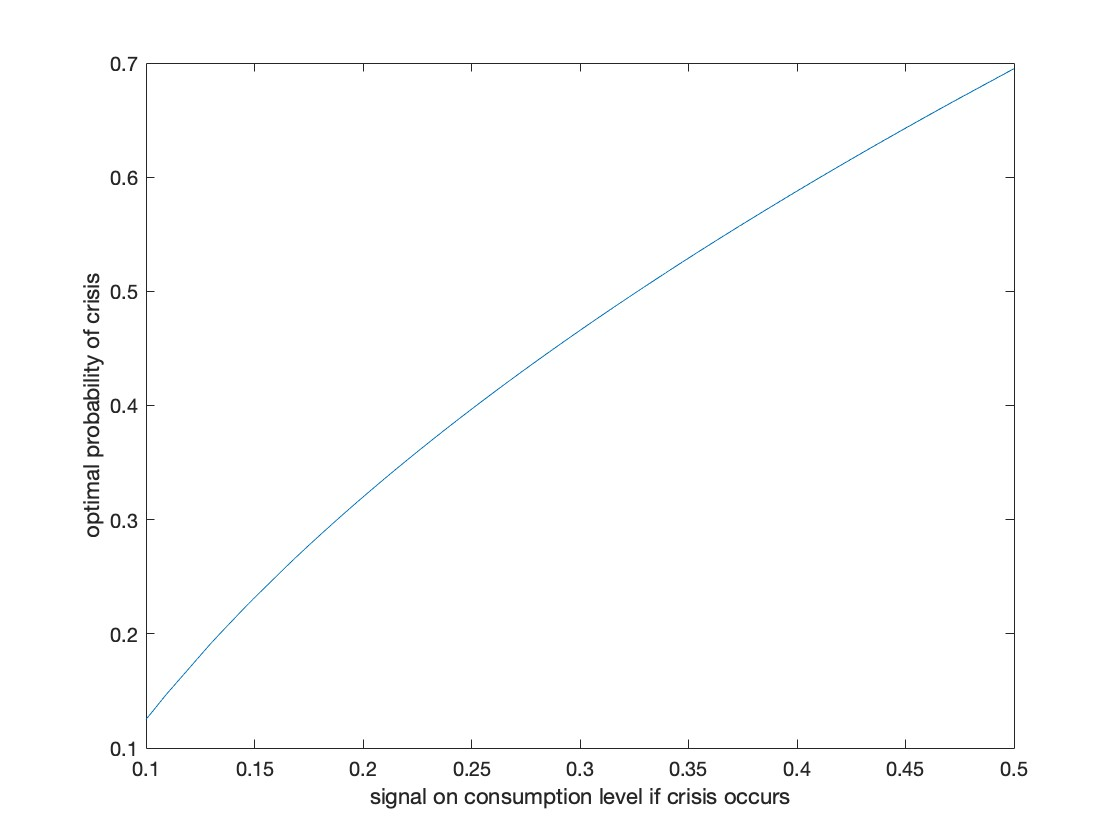
\includegraphics[width=0.75\linewidth]{images/Figure1base} 

}

\caption{Optimal probability of crisis as mapped from different beliefs about the optimal consumption level}\label{fig:Fig 3.1}
\end{figure}

\hypertarget{voters}{%
\subsection*{Voters}\label{voters}}
\addcontentsline{toc}{subsection}{Voters}

Voters are assumed to be homogenous in all respects except their
beliefs; which are determined entirely by the private signals that they
receive. Besley \& Coate (1997) find that according to the median voter
result and the Condorcet Jury theorem, there is one ultimate winning
candidate which is the median voter. According to the median voter
theorem, if preferences are single peaked (which is implied by the
uniformly distributed private signals in this model which determine
beliefs) then the median voter will be the winning candidate in a global
democracy vote, if we assume voter sincerity and a democratic voting
system.\footnote{The median voter result was checked numerically and
  holds up to numerical precision.}

It is further assumed that voting is conducted according to simple
majority voting and that each candidate could be running for public
office. As such, voters are assumed to have a continuous choice set of
possible candidates which ranges across the different beliefs of
individuals in the economy exactly. Voting is thus endogenised, as the
winning candidate is the candidate that yields the highest expected
utility for every pairwise comparison (Buchholz \emph{et al.}, 2005)

To determine the winning candidate, each voter considers each pairwise
comparison between each individual's policy preferences. Voters are
assumed to know that candidates could only implement their preferred
policy. This is a realistic assumption as it follows from the assumption
that that candidates cannot credibly commit to any other policy other
than their own policy preference and voters know this. Policy
preferences are thus in this context their individual optimal
consumption point and how this maps onto their optimal probability of
crisis. Based on the pairwise comparison, the voter votes for the
individual which maximises their expected utility.

\hypertarget{consumption-choices-in-two-non-cooperative-democracies}{%
\section{Consumption choices in two non-cooperative
democracies}\label{consumption-choices-in-two-non-cooperative-democracies}}

\emph{(approx 731)}

The primary concern in this thesis is to model the failure to
co-ordinate environmental agreements between two countries. This is
modelled in a similar way as Buchholz \emph{et al.} (2005), but only
gives consideration to the non-cooperative result. We assume that there
are two countries which are a partition of the global democracy
population and function independently of one another. The key mechanism
is that each country independently determines their own consumption
value (as chosen by the winning candidate for each country upon which
was voted independently), but the probability of a global climate crisis
is determined by the average consumption level across the two countries.
There is a discrepancy between voting conducted unilaterally and
ultimately facing the joint consequence globally. Thus, consumers in a
given country do not fully internalize the costs and risks of their
consumption choices in the two-country setting.

\hypertarget{economy-1}{%
\subsection*{Economy}\label{economy-1}}
\addcontentsline{toc}{subsection}{Economy}

To develop the model set-up further, the impact of another country's
consumption level on the optimal level of consumption is incorporated.
Accordingly, this model specification introduces two countries; country
A and country B. The implications of a two-country model which considers
the interdependence between countries is more realistic. A prime example
is the consideration of the impact of an IEA, as considered in Buchholz
\emph{et al.} (2005).

\hypertarget{consumers-1}{%
\subsection*{Consumers}\label{consumers-1}}
\addcontentsline{toc}{subsection}{Consumers}

As in the global democracy model, individuals in each country receive
private signals \(\hat{\underline{c}}_k\) which determine their optimal
level of consumption. These private signals are drawn again from a
distribution between \(c_L\) and \(c_H\), and are identically
distributed in each country unless adjustable parameters are altered to
create asymmetries. Individuals in the global economy are split into two
different country populations according to a stochastic assignment,
after each individual has received their private signals. Each
individual is divided probabilistically into either country A or country
B to ensure random splitting.

We study two dimensions of asymmetries in this model specification,
namely in the relative size and bias in the beliefs of the countries.
Variations in relative country size can be implemented by selecting a
value between 0 and 0.5. The higher the relative country size value, the
larger country A's population size is relative to country B. Variations
in belief bias can be implemented by selecting a value between 0 and
0.9. The higher the belief bias value, the more likely that those
individuals who receive higher private signals are to be assigned to
country A, and thus the more optimistic on average the beliefs are in
country A.

\hypertarget{voters-1}{%
\subsection*{Voters}\label{voters-1}}
\addcontentsline{toc}{subsection}{Voters}

As in the global democracy, the expected utilities for every possible
candidate are computed under the assumption that each citizen runs for
election and promises to implement their own ideal consumption level if
elected. Accordingly, each voter considers any pairwise competition
based on their expected utility and their own belief about \(\tilde{c}\)
as formed due to their private signal \(\hat{\underline{c}}_k\).

Thereafter, the mutual best responses for each country given what the
other country's consumption level is are determined. Each country's
citizens vote for the candidate in their respective country that will
yield the best response given how the other country votes to maximise
expected utility. For example, if country A is biased to consume at a
high level, then it would be a best response for country B to consume at
a lower level to reduce the probability of crisis to be closer to
country B's optimal probability of crisis. The Nash equilibrium in the
two-country model is determined using Matlab's built-in optimisers.

In each country, each individual has a best response function and votes
for the candidate that maximises their expected utility, conditional on
the other country's consumption level as well as their own consumption
level. However, albeit that the other country's consumption level is
taken as given, individuals do not fully internalise the joint impact of
both countries' average consumption on the probability of crisis.

In the case of strategic considerations that are not fully internalised,
there are two main findings. Non-cooperative results between two parties
are found to be worse than cooperative results, and Nash bargaining
results are found to lie somewhere in between these two polarised
results. Thus the focus of this paper is to analyze how the
non-cooperative results depend on asymmetries which Buchholz \emph{et
al.} (2005) do not study, and leave the bargaining results which their
paper investigates for future research.

\hypertarget{results-and-discussion}{%
\section{Results and discussion}\label{results-and-discussion}}

\emph{(1130)}

To analyse whether a lack of co-operation between two countries is
harmful for environmental policies and mitigating the probability of
climate crisis in the political economy, the global democracy model is
compared to three variations of the two-country case. Buchholz \emph{et
al.} (2005) compares the isolationist case (of one country which
implements climate policies unilaterally) against the bargaining case
(with an IEA implemented between two countries) to analyse the impact of
IEAs on environmental policy. Similarly, this paper compares the global
democracy of one voter population with a uniform distribution of beliefs
against the Nash equilibrium solution from the best response functions
from the two-country case. This result is found in the case of two
countries which do not have an IEA but instead reach non-cooperative
Nash results with three variations; namely the symmetric country size
model, the asymmetric country size model, and the asymmetric bias model.

\hypertarget{symmetric-country-size-model-results}{%
\subsection{Symmetric country size model
results}\label{symmetric-country-size-model-results}}

In this model variation, the share of each country's population is
approximately symmetric, as the adjustable parameter of relative country
size is set to 0.5. The population size in our estimation for country A
is 484 and 516 for country B. There is no bias introduced in this model.
The kernel density function in Figure 5.1 shows that the beliefs for
both countries have approximately the same distribution across optimal
probabilities of crisis. The functions overlap almost identically, with
minor exception at the left-hand tail and a slight discrepancy at the
approximate median value. The median optimal probability of crisis for
both countries is approximately 0.45 (Figure 5.1). Therefore, between
countries beliefs are not substantially different.

Figure 5.2 shows that when the population is split into two similarly
sized populations, each country's best response is to consume at higher
levels compared to the global democracy point. The Nash equilibrium
point is much higher at \(c_1=1.2134\) for each country. Thus, the
non-cooperative Nash outcome is that both countries consume more in the
first period.

\begin{figure}[H]

{\centering 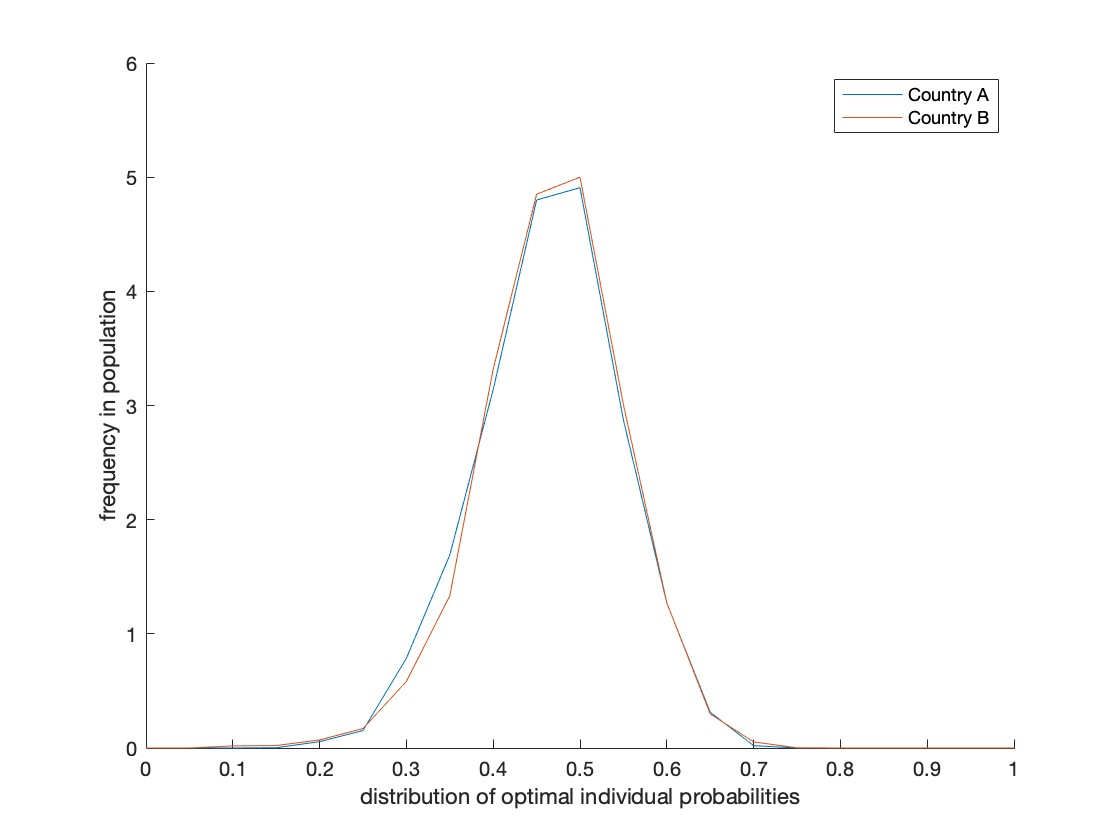
\includegraphics[width=0.75\linewidth]{images/Fig4_0.5Size0Bias} 

}

\caption{Symmetric country size model: Kernel density function of the distribution of the optimal probabilty of crisis and frequency thereof across individuals in country A and country B}\label{fig:Fig 5.1}
\end{figure}

\begin{figure}[H]

{\centering 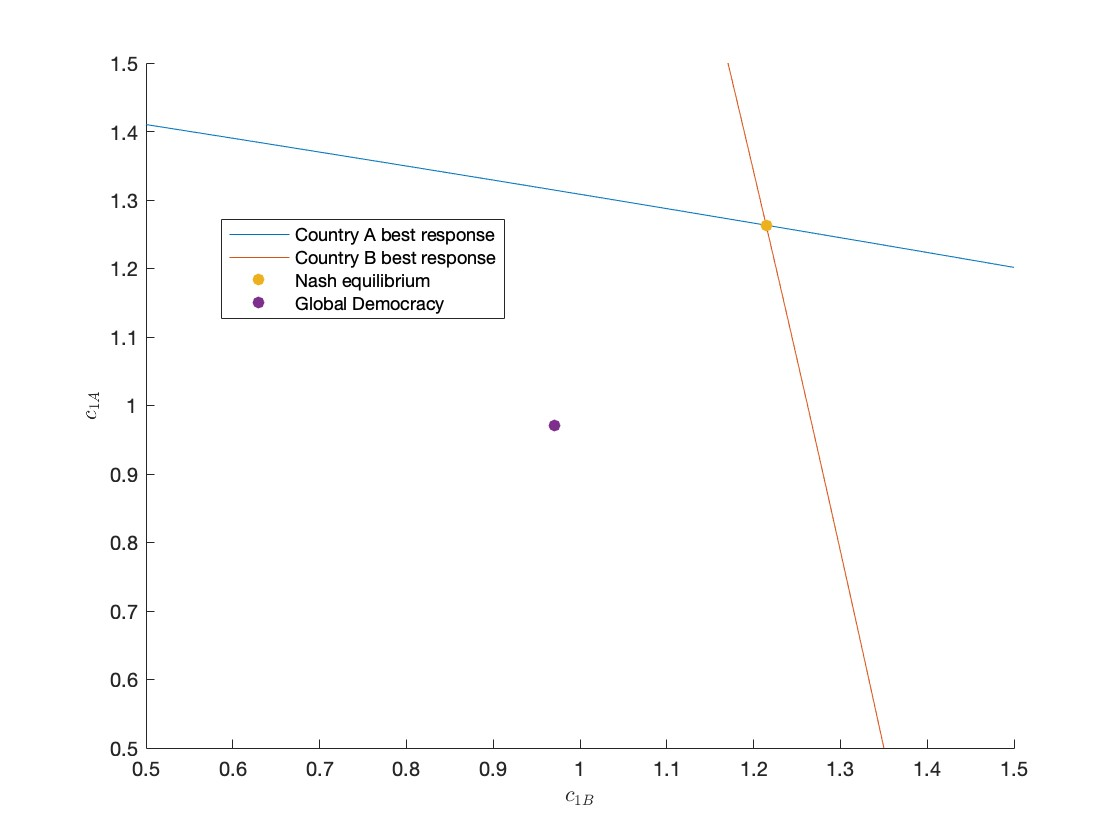
\includegraphics[width=0.75\linewidth]{images/Fig2_0.5Size0Bias} 

}

\caption{Best response functions for symmetric country size model compared to global democracy}\label{fig:Fig 5.2}
\end{figure}

\hypertarget{asymmetric-country-size-model-results}{%
\subsection{Asymmetric country size model
results}\label{asymmetric-country-size-model-results}}

In this variation of the two-country model, the adjustable parameter of
relative country size is set to 0.1. The population sizes in the
estimation are 104 in country A and 896 in country B. Figure 5.3 shows
that beliefs are substantially similar across the distribution of
optimal individual probabilities between countries. Albeit that there
are slight discrepancies in the curvature between countries in Figure
5.3, both countries' kernel density functions have the same approximate
shape and share an approximate median optimal probability of crisis of
0.45.

\begin{figure}[H]

{\centering 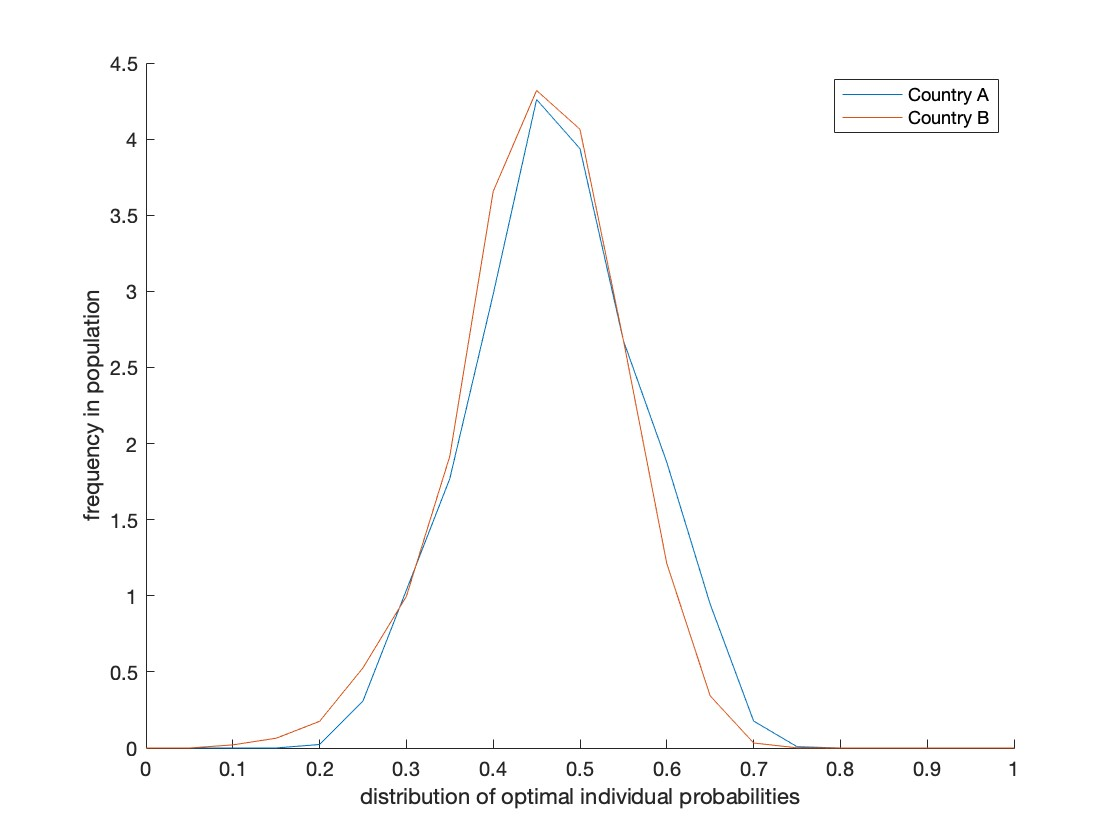
\includegraphics[width=0.75\linewidth]{images/Fig4_0.1Size0Bias} 

}

\caption{Asymmetric country size model: Kernel density function of the distribution of the optimal probabilty of crisis and frequency thereof across individuals in country A and country B}\label{fig:Fig 5.3}
\end{figure}

As is shown in Figure 5.4, when country A has a significantly smaller
population size it is a best response for country A to consume at the
highest threshold \(c_{1A}=c_H=1.5\) that is possible, irrespective of
the consumption level that country B chooses. On the other hand, country
B's best response is to consume at a significantly lower level of
approximately \(c_{1B}=1\) irrespective of what country A consumes. The
Nash equilibrium result in the case of a larger country B and a smaller
country A leads country A to consume much more than the global democracy
case, and country B to consume only slightly more. Notably, country A
consumes 0.5 more than country B in the first period, which yields a
significant imbalance as a result of a large size difference between the
countries.

\begin{figure}[H]

{\centering 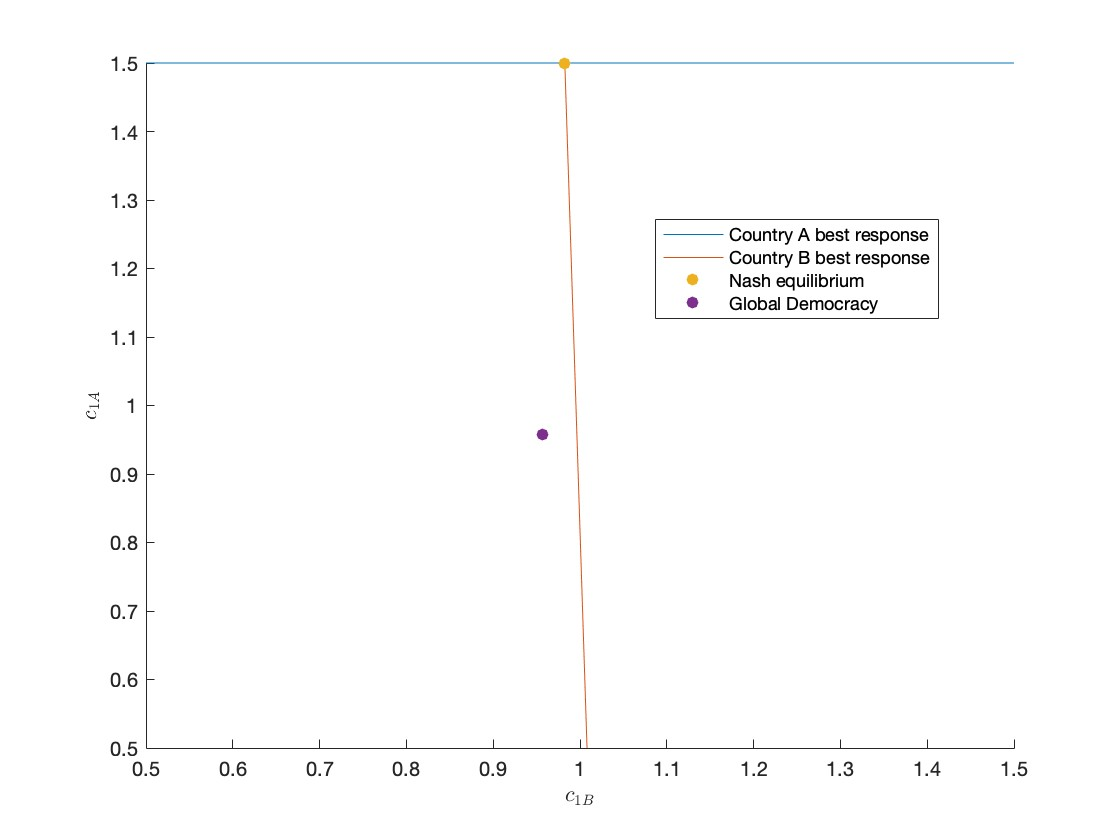
\includegraphics[width=0.75\linewidth]{images/Fig2_0.1Size0Bias} 

}

\caption{Best response functions for asymmetric country size model compared to global democracy}\label{fig:Fig 5.4}
\end{figure}

\hypertarget{asymmetric-bias-model-results}{%
\subsection{Asymmetric bias model
results}\label{asymmetric-bias-model-results}}

In our final variation model, a change in the adjustable parameter for
bias is implemented. Bias is set to a value of 0.9, and increased from a
value of zero for the previous two model specifications. The population
is kept symmetric (country relative size parameter is set at 0.5) and is
523 for country A and 477 for country B in this estimation. Figure 5.5
shows a significant discrepancy between beliefs in the population of
country A and country B. Country A's distribution of beliefs about the
optimal probability of crisis have a higher frequency of approximately 6
individuals at the median probability of 0.5. On the other hand, country
B's median probability is approximately 0.4 with a frequency of just
less than 5. Thus, country B's distribution of beliefs are lower on
average compared to country A.

\begin{figure}[H]

{\centering 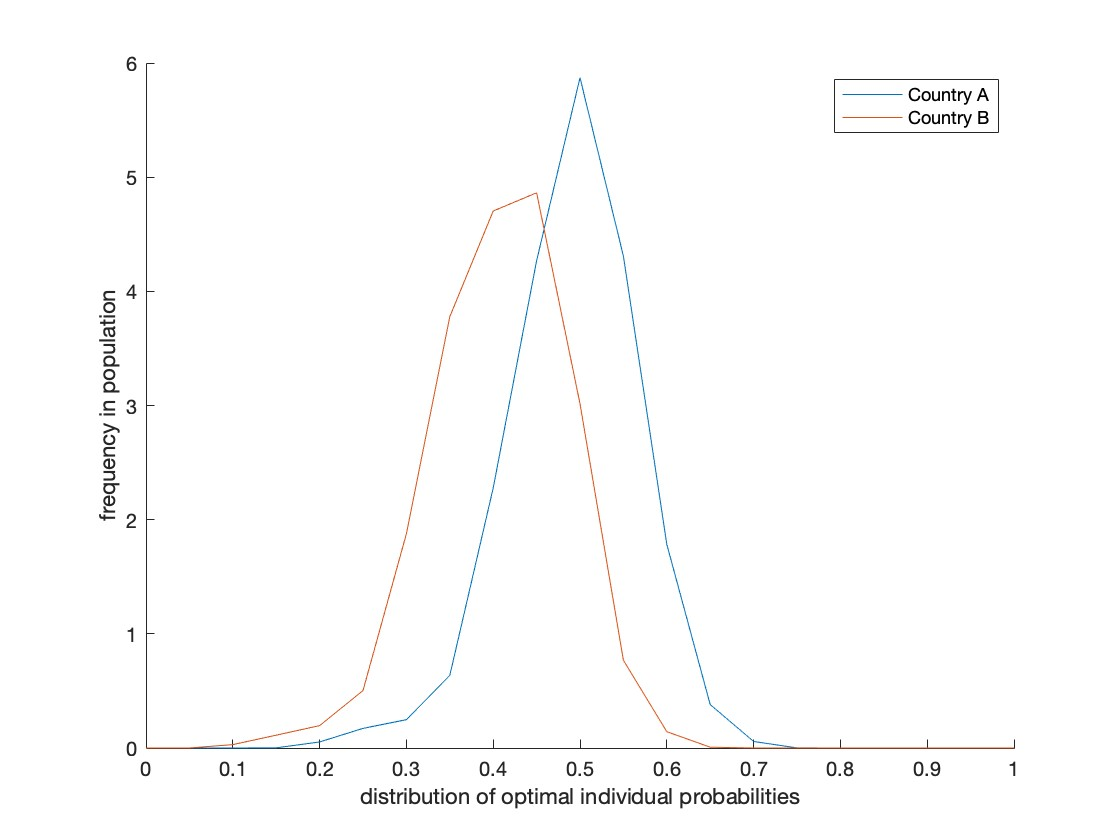
\includegraphics[width=0.75\linewidth]{images/Fig4_0.5Size0.9Bias} 

}

\caption{Asymmetric country bias model: Kernel density function of the distribution of the optimal probabilty of crisis and frequency thereof across individuals in country A and country B}\label{fig:Fig 5.5}
\end{figure}
\begin{figure}[H]

{\centering 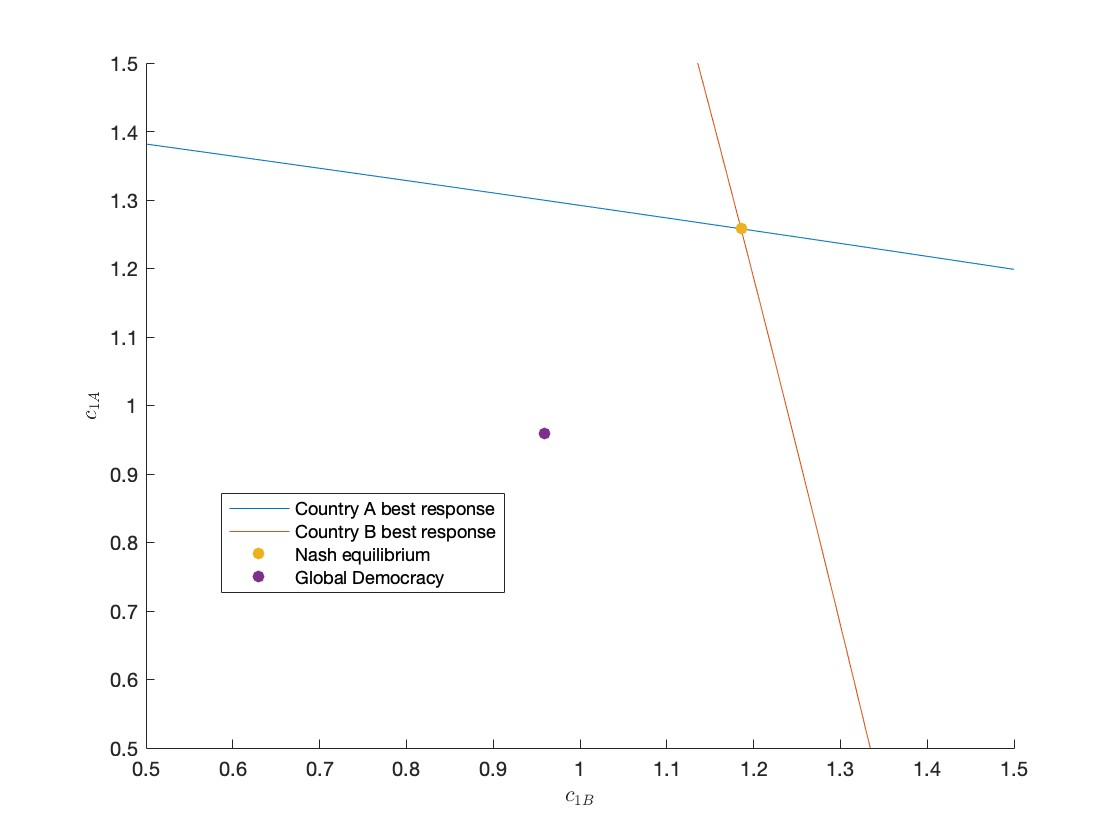
\includegraphics[width=0.75\linewidth]{images/Fig2_0.5Size0.9Bias} 

}

\caption{Best response functions for assymetric bias model compared to global democracy}\label{fig:Fig 5.6}
\end{figure}

Figure 5.6 shows that the best response functions in the non-cooperative
case between a country with relatively higher bias and another with
unbiased beliefs leads to a much higher consumption level. For both
countries in this model, consumption in the first period is
\(c_1=1.2234\).

\hypertarget{discussion}{%
\subsection{Discussion}\label{discussion}}

The main objective of the comparison across model variations is to
determine whether imbalances in relative country size and biased beliefs
are beneficial or harmful for advancing environmental policy objectives.
Buchholz \emph{et al} (2005) reaches an analytical result in which
voters may be incentivised to vote for less green candidates in order to
improve their own country's bargaining position when there is an IEA.
This implies that unless there is full co-operation, any bargaining
outcome is bad for environmental policy and the probability of a climate
crisis. Besley \& Coate (1997) also suggest that non-cooperation with
other countries may yield a greater expected utility than if
co-operation occurs.

Buchholz \emph{et al.} (2005) provide a possible reason for this ``of
transboundary pollution, where the economic activities of one country
have negative effects on other regions. Since national governments do
not take these externalities into account when they decide on their
environmental policies, their non-cooperative strategies generally lead
to an inefficiently poor state of the ecological system.'' Buchholz
\emph{et al.} (2005) finds that compared to the median outcome,
co-operating governments care less about environmental outcomes

Firstly, it is clear from the results discussed that introducing
asymmetries between countries related to relative country size and
biased beliefs leads to higher period one consumption for both countries
in all cases. The extent of increased consumption varies across the
different model specifications. Higher consumption levels are only
optimal if beliefs are increased and it is believed that the climate
crisis will not be too severe.

As evidenced in Table 1, the global democracy model's beliefs are
approximately equal to the beliefs in both the symmetric and asymmetric
country size models. The inability for voters to account for the joint
impact of both country A and country B's consumption on the probability
of crisis results in voters voting for higher consumption despite it
leading to an increased likelihood of crisis. Thus, the Nash equilibrium
result that arises from the best response functions of each country is
sub-optimal and Pareto inefficient.

Secondly, different asymmetries lead to different consumption
imbalances. For the symmetric size model, country A's population of 484
is smaller than country B's population of 516. The consumption levels of
country A exceed those of country B, and country A's period one
consumption is 1.2601 and country B's period one consumption is 1.0363
(Table 1). A similar result arises in the asymmetric size model, where
the significantly smaller country A can consume at the highest threshold
possible. Therefore, a smaller country has a best response function
which yields a greater expected utility for higher consumption levels
than for a relatively larger country.

On the other hand, in the asymmetric bias model, country A has a higher
population than country B in similar relative proportions as the
symmetric size model (country A's population is 523 and country B's
population is 477 in the asymmetric model estimation) but country A's
consumption level is higher than country B. This can be accounted for
due to the higher level of biased beliefs in country A than in country
B. Thus, due to country A having more voters that believe that the
climate crisis will not be too severe, means it is a best response on
average for voters in country A to vote in higher consumption levels
than country B.

Therefore, in these non-cooperative model results it is demonstrated
that introducing two-country interdependence yields higher consumption
levels for both countries which accordingly increases the probability of
crisis which is detrimental to both countries. Albeit the higher
probability of crisis that arises for the asymmetric model is not much
higher than the global democracy case, as the former has yields a
probability of 0.5363 and the latter a probability of 0.4499 (Table 1).
Therefore, the country with a significantly smaller population and
without bias can take advantage of their smaller size to consume at
higher levels without incurring a substantially higher risk of crisis.

Whereas, if the country has beliefs which are biased to be higher on
average then such a country can consume more than another country.
However, the risk of a situation in which countries are approximately
symmetric in size and asymmetric in beliefs yields the highest
probability of crisis across the model variations considered in this
thesis.

Both countries in the asymmetric country size model consume more in
period 1 which could only be a better outcome in comparison to the
global democracy point (plotted on Figure 5.1) if both countries'
individuals believe that a higher probability of crisis is optimal.
However, there is not a substantial difference in beliefs from the
global democracy model in this model variation. The asymmetric country
size model only differs from the global democracy model in one aspect,
which is the country size. Thus, this outcome is slightly less efficient
than the global democracy case, as the probability of crisis in Nash
equilibrium is higher, as shown in Table 5.1. \emph{This implies that
voters vote in a candidate that is less green than their own policy
preferences, which provides support for the finding in Buchholz et al}

\newpage
\begin{center}
Table 5.1: Results for model variations to compare period one consumption and the probability of crisis across four different model variations
\end{center}

\begin{longtable}[]{@{}
  >{\raggedright\arraybackslash}p{(\columnwidth - 8\tabcolsep) * \real{0.1905}}
  >{\centering\arraybackslash}p{(\columnwidth - 8\tabcolsep) * \real{0.2381}}
  >{\centering\arraybackslash}p{(\columnwidth - 8\tabcolsep) * \real{0.2381}}
  >{\centering\arraybackslash}p{(\columnwidth - 8\tabcolsep) * \real{0.1667}}
  >{\centering\arraybackslash}p{(\columnwidth - 8\tabcolsep) * \real{0.1667}}@{}}
\toprule()
\begin{minipage}[b]{\linewidth}\raggedright
\end{minipage} & \begin{minipage}[b]{\linewidth}\centering
Global democracy
\end{minipage} & \begin{minipage}[b]{\linewidth}\centering
Symmetric size
\end{minipage} & \begin{minipage}[b]{\linewidth}\centering
Asymmetric size
\end{minipage} & \begin{minipage}[b]{\linewidth}\centering
Asymmetric bias
\end{minipage} \\
\midrule()
\endhead
Population size & 1000 & A 484 & A 104 & 523 \\
& & B 516 & B 896 & 477 \\
Consumption & 0.9499 & A 1.2601 & A 1.5000 & A 1.2781 \\
& 1.2234 & B 1.2134 & B 1.0363 & B 1.2234 \\
Beliefs median & 0.4499 & 0.4500 & 0.4500 & A 0.5000 \\
& & & & B 0.4000 \\
Actual crisis probability & 0.4499 & 0.7134 & 0.5363 & 0.7234 \\
\bottomrule()
\end{longtable}

A higher consumption point as a Nash equilibrium in this model is
sub-optimal and welfare-reducing for both countries. Moreover, it is not
a Pareto efficient outcome because it would be better for both countries
to consume less but due to imperfect co-operation, this outcome cannot
be achieved.

Table 5.1 shows that this final model yields both the highest period one
consumption for both country A and country B, as well as the highest
probability of crisis. Therefore, it seems that the worst outcome across
the four models considered is the asymmetric country bias situation, in
which two countries are approximately equal in size but one country
receives fundamentally different private signals about climate change.
In Figure 5.6, the Nash equilibrium consumption point is significantly
higher than the global democracy point.

However, to compare equal size and equal size plus bias, the difference
in Nash equilibrium points is not significantly different. Thus it is
worse to go from an asymmetric country size scenario to a two equal
sized country scenario compared to introducing bias into one country's
beliefs.

The probability of crisis in Nash equilibrium for this asymmetric bias
model variation is 0.7234, which is the optimal probability of crisis
for less than one individual in country A and no individuals in country
B. Similarly to the symmetric country size model, the optimal
consumption point and probability of crisis in the Nash equilibrium is
not Pareto efficient and is thus sub-optimal.

\hypertarget{conclusion}{%
\section{Conclusion}\label{conclusion}}

\begin{enumerate}
\def\labelenumi{(\arabic{enumi})}
\setcounter{enumi}{799}
\tightlist
\item
\end{enumerate}

Buchholz \emph{et al.} (2005) suggests to overcome the lack of
co-operation, could create mandatory side-payments that must be paid by
the country that induces pollution in the other country to the other
country to account for the negative externality which would adjust
voters and politicians payoffs to consider environmental degradation
more directly and thus lead to better co-operative outcomes. But in
their model they include the trade-off between domestic product and
environmental policies, so would not improve our models outcomes, would
require a different specification

\newpage

\hypertarget{references}{%
\section*{References}\label{references}}
\addcontentsline{toc}{section}{References}

Adler, M. D. \& Treich, N. Utilitarianism, prioritarianism, and
intergenerational equity: A cake eating model. \emph{Mathematical Social
Sciences}, 87(1):94-102.

Besley, T. \& Coate, S. 1997. An economic model of representative
democracy. \emph{Quarterly Journal of Economics}, 112(1):85-114.

Buchholz, W., Haupt, A. \& Peters, W. 2005. \emph{The Scandinavian
Journal of Economics}, 107(1):175-195.

Kumar, R. C. 2005. How to eat a cake of unknown size: A reconsideration.
\emph{Journal of Environmental Economics and Management}, 50(1):408-421.

Lemoine, D. \& Traeger, C. 2014. Watch Your Step: Optimal Policy in a
Tipping Climate. \emph{American Economic Journal: Economic Policy},
6(1):137-166.

Lohmann, S. 1994. Information Aggregation Through Costly Political
Action. \emph{The American Economic Review}, 84(3):518-530.

Loury, G. C. 1978. The Optimal Exploitation of an Unknown Reserve.
\emph{The Review of Economic Studies}, 45(3):621-636.

Piketty, T. 1999. The information-aggregation approach to political
institutions. \emph{European Economic Review}, 43(1):791-800.

Pindyck, R. S. 1978. The Optimal Exploration and Production of
Nonrenewable Resources. \emph{Jorunal of Political Economy},
86(5):841-861.

Razin, R. 2003. Signaling and election motivations in a voting model
with common values and responsive candidates. \emph{Econometrica},
71(4):1083-1119.

\bibliography{Tex/ref}





\end{document}
